%%%%%%%%%%%%%%%%%%%%%%%%%%%%%%%%%%%%%%%%%%%%%%%%%%%%%%%%%%%%%%%%%%%%%%%%%%%%%%
%% Lecture 3: Introduction to Supervised Learning.
%% Compile with: latexmk -pdf lecture03
%% Handout (overlays collapsed, solutions shown): latexmk -pdf lecture03-handout
%% Speaker notes: add the notes option to \usepackage below.
%%
%% Figures: ../codes/l03_figures.py (run with uv run codes/l03_figures.py).
%% Based on the 2025 slides of Stevan Rudinac and on Lecture 4 of Andreas
%% Mueller's Applied Machine Learning course (Columbia University, 2017).
%%%%%%%%%%%%%%%%%%%%%%%%%%%%%%%%%%%%%%%%%%%%%%%%%%%%%%%%%%%%%%%%%%%%%%%%%%%%%%

% lecture03-handout.tex defines \sibhandout before reading this file.
\ifdefined\sibhandout
  \documentclass[handout,aspectratio=169,t,9pt]{beamer}
  \usepackage[macros,solutions]{siblecture2026}
\else
  \documentclass[aspectratio=169,t,9pt]{beamer}
  \usepackage[macros]{siblecture2026}
\fi

% Everything specific to this course goes here.
\graphicspath{{figures/}{../images/}}
\usepackage{booktabs}
\usepackage{listings}
\lstset{language=Python,
        basicstyle=\ttfamily\footnotesize,
        keywordstyle=\color{sibTwo}\bfseries,
        stringstyle=\color{sibOne},
        commentstyle=\color{uvaDarkGrey},
        backgroundcolor=\color{uvaGrey},
        columns=fullflexible,keepspaces=true,showstringspaces=false,
        frame=none,xleftmargin=4pt,xrightmargin=4pt,
        aboveskip=4pt,belowskip=4pt}
\usetikzlibrary{positioning,arrows.meta}

% A row of data blocks for the split diagrams: \datarow{y}{list of
% start/end/fill/label}.
\tikzset{blk/.style={draw=white,thick,minimum height=0.55cm,font=\scriptsize,
                     text=white,inner sep=0pt}}
\newcommand{\datablock}[5]{%
  \fill[#4] (#1,#3) rectangle (#2,#3+0.55);
  \draw[white,thick] (#1,#3) rectangle (#2,#3+0.55);
  \node[font=\scriptsize,text=white] at ({(#1+#2)/2},#3+0.275) {#5};}
\colorlet{trainc}{sibTwo}
\colorlet{valc}{sibThree}
\colorlet{testc}{sibOne}

%%%%%%%%%%%%%%%%%%%%%%%%%%%%%%%%%%%%%%%%%%%%%%%%%%%%%%%%%%%%%%%%%%%%%%%%%%%%%%

\course{Machine Learning with Python}
\coursesubtitle{Minor Amsterdam Data Science and Artificial Intelligence}
\term{Fall 2026}

\lectureno{3}
\title{Introduction to Supervised Learning}
\subtitle{Nearest neighbors, and how to choose a model honestly}
\author{\c{S}. \.{I}lker Birbil}
\institute{University of Amsterdam}
\date{November 2, 2026}
\contact{s.i.birbil@uva.nl}

% ============================================================
\begin{document}
% ============================================================

\sibtitleframe

\sibtocframe[Lecture overview]

\begin{frame}{What you should be able to do afterwards}
  \begin{objectives}
    \item Explain how $k$-nearest neighbors makes a prediction.
    \item Train and test a model with scikit-learn.
    \item Explain how $k$ controls underfitting and overfitting.
    \item Choose a model setting with cross-validation and grid search.
  \end{objectives}

  \vfill
  \begin{recap}
    Plot the data before modeling it: plots reveal wrong types, mixed
    definitions and defaults that summary numbers hide.
  \end{recap}
\end{frame}

% ==================================================================
\section{Nearest Neighbors}
% ==================================================================

\begin{frame}{The task}
  \begin{columns}[T,onlytextwidth]
    \begin{column}{0.58\textwidth}
      \centering
      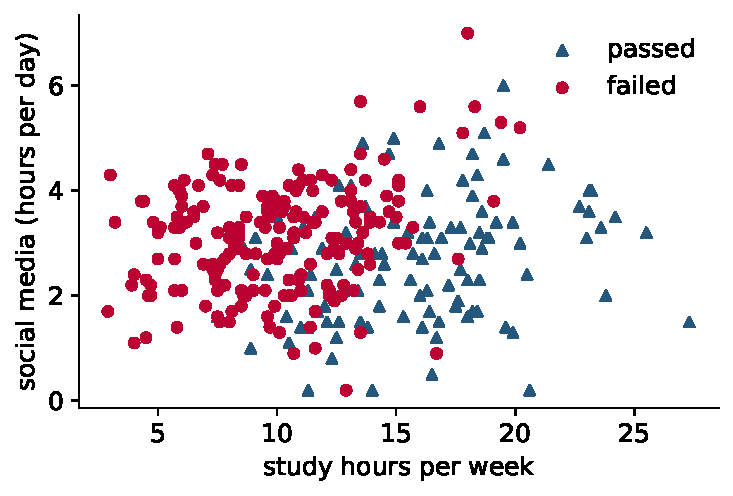
\includegraphics[width=\linewidth]{l03_task.pdf}
    \end{column}
    \begin{column}{0.38\textwidth}
      \vspace{0.3cm}
      \begin{itemize}
        \item 300 students from the course survey
        \item \textbf{Features:} study hours, social media hours
        \item \textbf{Label:} passed or failed
        \item A \highlight{classification} problem
      \end{itemize}
    \end{column}
  \end{columns}

  \note{Two features only, so that we can draw everything.  The same ideas
    work with any number of features.  About 36\% of the students passed.}
\end{frame}

\begin{frame}{Ask the neighbors}
  \centering
  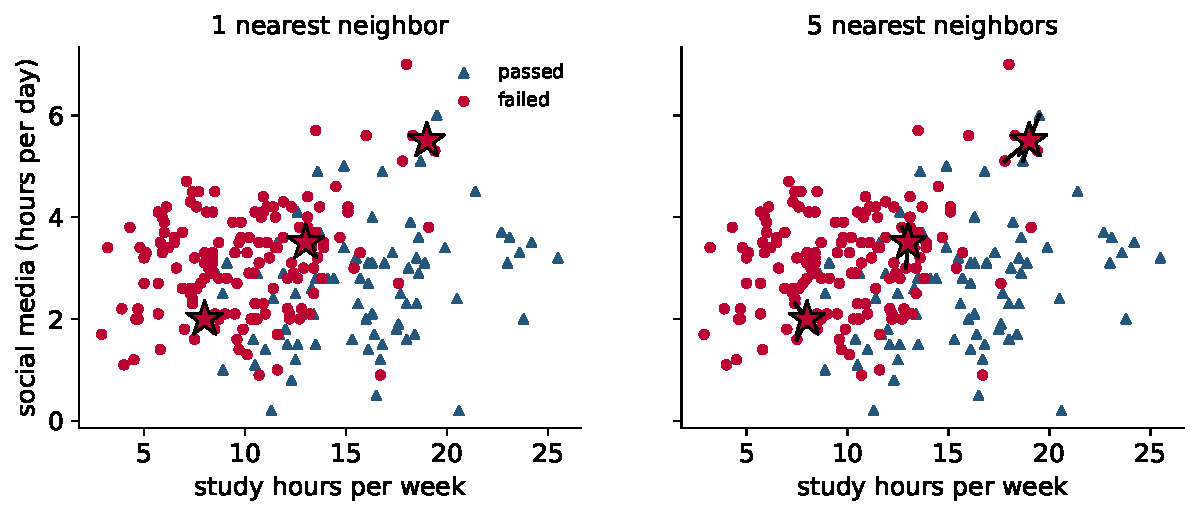
\includegraphics[height=4.4cm]{l03_neighbors.pdf}

  \raggedright
  \textbf{1-NN:} copy the label of the closest student. \quad
  \textbf{$k$-NN:} majority vote among the $k$ closest.

  \note{The stars are three new students.  ``Closest'' means the shortest
    straight line in the plot.  With one neighbor, the middle star depends
    on a single student; with five, the vote is more stable.}
\end{frame}

\begin{frame}{Distance depends on the units}
  \centering
  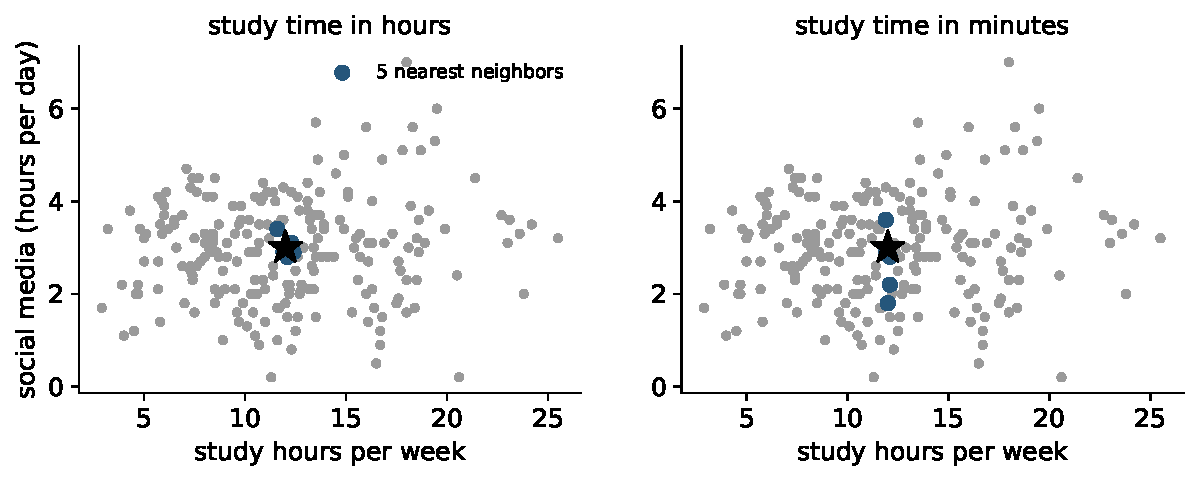
\includegraphics[height=4.4cm]{l03_units.pdf}

  \vfill
  \begin{keypoint}{Watch out}
    In minutes, study time dominates the distance, and social media
    hardly counts.  Lecture~6 shows how to put features on one scale.
  \end{keypoint}

  \note{Same students, same star.  Only the unit of study time changes:
    hours on the left, minutes on the right.  On the right the five nearest
    neighbors are simply the students with almost the same study time.}
\end{frame}

\begin{frame}{Training data and test data}
  \vspace{0.3cm}
  \centering
  \begin{tikzpicture}
    \datablock{0}{9}{0}{trainc}{training set (75\%): the model learns from it}
    \datablock{9}{12}{0}{testc}{test set (25\%)}
  \end{tikzpicture}

  \vspace{0.6cm}
  \raggedright
  \begin{itemize}
    \item Split the data \highlight{at random}, before anything else.
    \item Use the test set \highlight{once}, to estimate performance on new
          data.
  \end{itemize}

  \note{This is the test set promised in Lecture 1.  The model never sees
    the test labels during training, so the test score imitates what
    happens on new students.}
\end{frame}

\begin{frame}[fragile]{$k$-NN in scikit-learn}
  \begin{lstlisting}
from sklearn.model_selection import train_test_split
from sklearn.neighbors import KNeighborsClassifier

X = df[["study_hours", "social_media_hours"]]
y = df["passed"]
X_train, X_test, y_train, y_test = train_test_split(X, y, random_state=0)

knn = KNeighborsClassifier(n_neighbors=5)
knn.fit(X_train, y_train)       # learn from the training set
knn.predict(X_test)             # predicted labels
knn.score(X_test, y_test)       # accuracy: 0.80
  \end{lstlisting}

  \vfill
  \begin{takeaway}
    Every model in scikit-learn works the same way: \texttt{fit},
    \texttt{predict}, \texttt{score}.
  \end{takeaway}

  \note{Accuracy is the share of correct predictions.  Lecture 9 shows when
    accuracy is not enough.  random\_state fixes the random split, so that
    everybody gets the same numbers.}
\end{frame}

\begin{frame}{The effect of $k$}
  \centering
  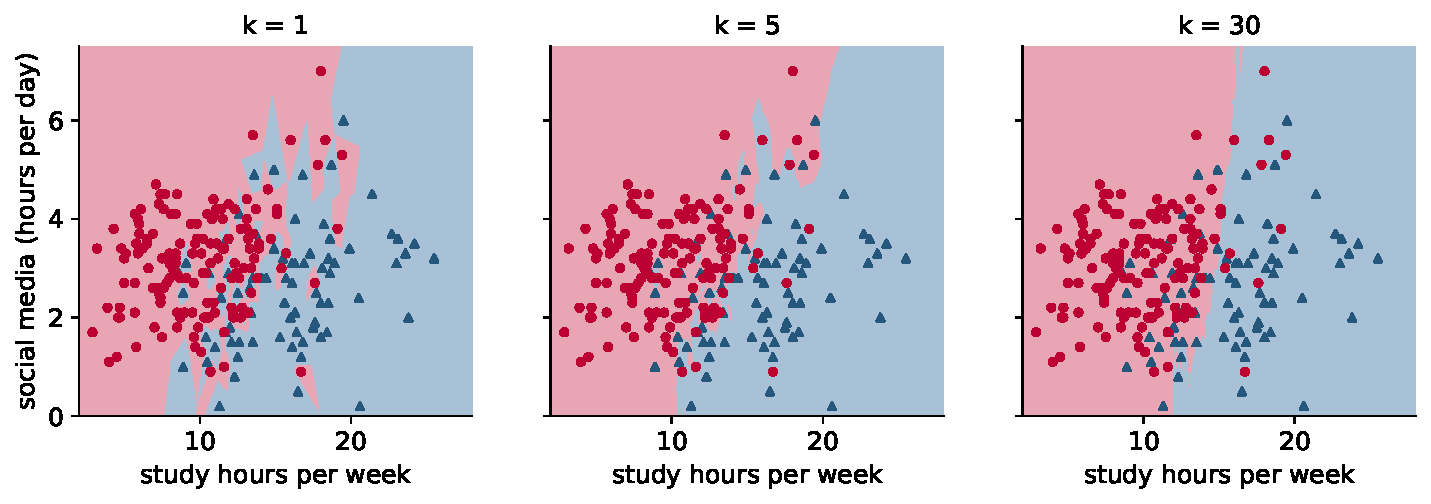
\includegraphics[width=\textwidth]{l03_boundaries.pdf}

  \vspace{0.2cm}
  \raggedright
  Small $k$: a ragged boundary that follows single students.
  Large $k$: a smooth boundary.

  \note{The background shows the prediction for every possible student:
    blue for passed, red for failed.  The line where the color changes is
    the decision boundary.}
\end{frame}

\begin{frame}{Accuracy against $k$}
  \begin{columns}[T,onlytextwidth]
    \begin{column}{0.58\textwidth}
      \centering
      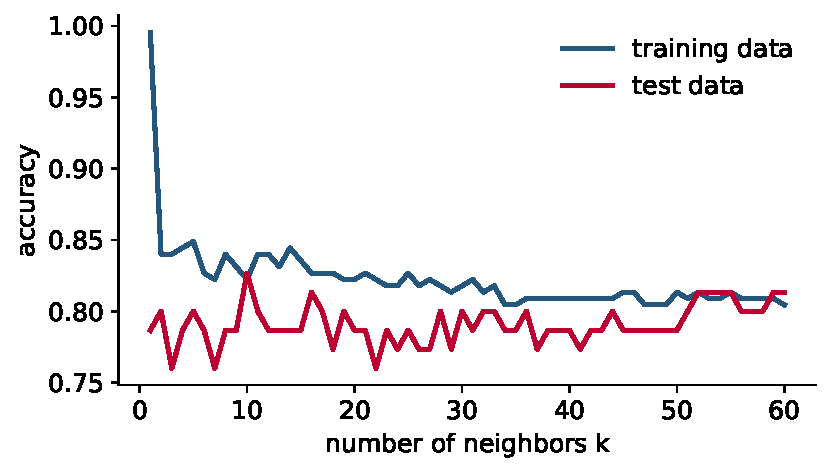
\includegraphics[width=\linewidth]{l03_accuracy_k.pdf}
    \end{column}
    \begin{column}{0.38\textwidth}
      \vspace{0.3cm}
      \begin{itemize}
        \item $k = 1$: training $99.6\%$, test $79\%$
        \item Training accuracy falls as $k$ grows.
        \item Test accuracy is what counts.
      \end{itemize}
    \end{column}
  \end{columns}

  \note{1-NN is not exactly 100\% on the training data because two
    students have the same answers but different outcomes.  The test curve
    is noisy: only 75 test students.}
\end{frame}

\begin{frame}{The sweet spot}
  \begin{columns}[T,onlytextwidth]
    \begin{column}{0.58\textwidth}
      \centering
      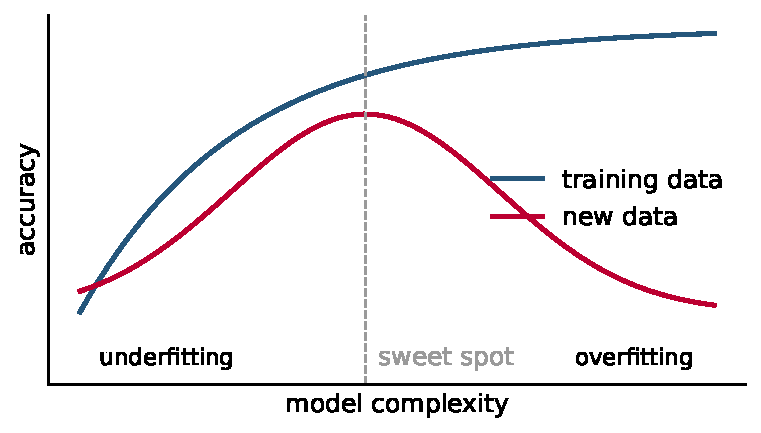
\includegraphics[height=3.9cm]{l03_sweetspot.pdf}
    \end{column}
    \begin{column}{0.38\textwidth}
      \vspace{0.3cm}
      \begin{itemize}
        \item Small $k$ = complex model
        \item Large $k$ = simple model
        \item The best $k$ lies in between.
      \end{itemize}
    \end{column}
  \end{columns}

  \vspace{0.2cm}
  \begin{keypoint}{Hyperparameter}
    A setting that we choose and the model does not learn, such as $k$.
  \end{keypoint}

  \note{The same picture holds for almost every model in the course; only
    the dial that controls complexity changes.}
\end{frame}

\begin{frame}{$k$-NN for regression}
  \centering
  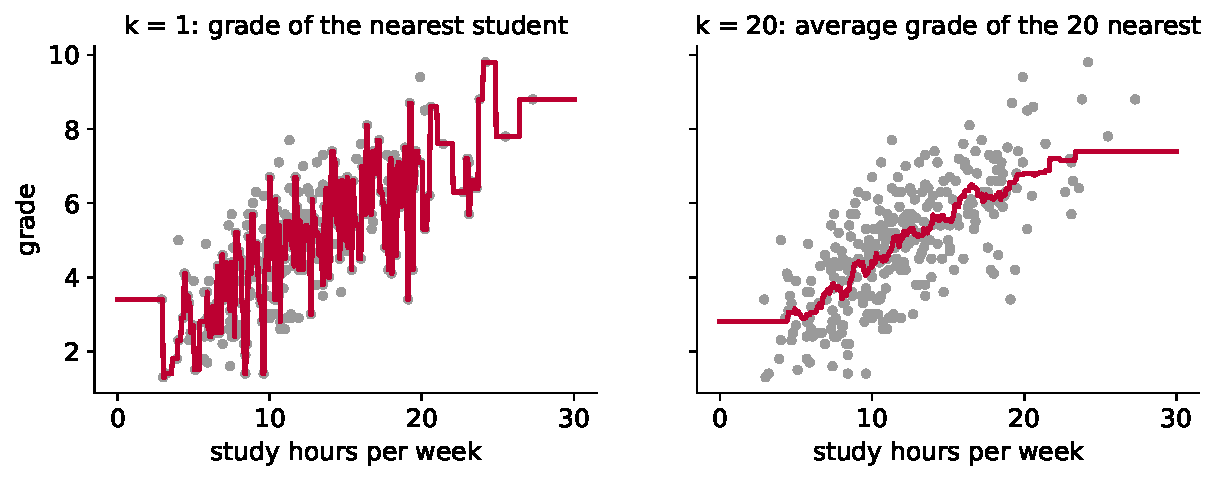
\includegraphics[height=4.3cm]{l03_regression.pdf}

  \raggedright
  Predict a \highlight{number}: the average grade of the $k$ nearest
  students.  In scikit-learn: \texttt{KNeighborsRegressor}.

  \note{Here the only feature is study hours.  k = 1 follows every student
    and overfits; k = 20 gives a smooth curve.  Lecture 4 fits a straight
    line instead.}
\end{frame}

\begin{frame}{Check your understanding}
  \begin{exercise}[think about $k$]
    \begin{enumerate}[label=(\alph*),itemsep=2pt,topsep=3pt]
      \item What is the training accuracy of 1-NN, roughly?
      \item Does a larger $k$ give a simpler or a more complex boundary?
      \item What does $k$-NN predict when $k$ equals the number of
            training students?
    \end{enumerate}
  \end{exercise}

  \begin{solution}
    (a) About 100\%: each student is its own nearest neighbor.
    (b) Simpler.
    (c) The majority class for everybody: here ``failed'', which is
    correct for about 64\% of the students.
  \end{solution}

  \note{Answer (c) is a baseline, as in Lecture 1: any useful model must
    beat 64\%.}
\end{frame}

% ==================================================================
\section{Choosing a Model}
% ==================================================================

\begin{frame}{The first session in one slide}
  \vspace{0.3cm}
  \begin{recap}[Where we are]
    \begin{itemize}
      \item $k$-NN predicts from the $k$ closest training examples.
      \item Train on the training set; test on the test set.
      \item $k$ controls complexity: too small overfits, too large
            underfits.
    \end{itemize}
  \end{recap}

  \vspace{0.6cm}
  Now: \highlight{how do we choose $k$}?
\end{frame}

\begin{frame}{Do not choose $k$ on the test set}
  \vspace{0.3cm}
  \begin{columns}[T,onlytextwidth]
    \begin{column}{0.48\textwidth}
      \begin{itemize}
        \item Best $k$ on our test set: $k = 10$, accuracy $83\%$.
        \item But we \emph{chose} $k$ because it scored best there.
        \item So $83\%$ is too optimistic for new students.
      \end{itemize}
    \end{column}
    \begin{column}{0.48\textwidth}
      \begin{keypoint}{Rule}
        The test set is for the final check only.  Choosing anything with
        it turns it into training data.
      \end{keypoint}
    \end{column}
  \end{columns}

  \note{Analogy: a teacher who shows the exam questions in class can no
    longer use the exam to measure what students learned.  Later in this
    lecture the honest procedure gives 79\% on the same test set.}
\end{frame}

\begin{frame}{Training, validation and test sets}
  \vspace{0.3cm}
  \centering
  \begin{tikzpicture}
    \datablock{0}{6}{0}{trainc}{training: fit the model}
    \datablock{6}{9}{0}{valc}{validation: choose $k$}
    \datablock{9}{12}{0}{testc}{test: final check}
  \end{tikzpicture}

  \vspace{0.6cm}
  \raggedright
  \begin{itemize}
    \item Try every $k$ on the training set; compare them on the
          validation set.
    \item Refit the best $k$ on training + validation; score once on the
          test set.
  \end{itemize}

  \vfill
  \muted{Simple and fast, but the result depends on one random split.}
\end{frame}

\begin{frame}{Cross-validation}
  \vspace{0.2cm}
  \centering
  \begin{tikzpicture}[yscale=0.8]
    \foreach \r in {0,...,4} {
      \foreach \c in {0,...,4} {
        \ifnum\c=\r
          \datablock{\c*1.8}{\c*1.8+1.8}{-\r*0.75}{valc}{validation}
        \else
          \datablock{\c*1.8}{\c*1.8+1.8}{-\r*0.75}{trainc}{training}
        \fi
      }
      \node[font=\scriptsize,anchor=east] at (-0.1,-\r*0.75+0.275)
        {split \the\numexpr\r+1\relax};
    }
    \datablock{9.3}{11.3}{-1.5}{testc}{test}
    \node[font=\scriptsize,text=sib@mute] at (10.3,-1.95) {kept apart};
  \end{tikzpicture}

  \vspace{0.3cm}
  \raggedright
  Split the training data into 5 \textbf{folds}; each fold is the validation
  set once.  Average the 5 scores.

  \note{Every training student is used for validation exactly once.  The
    average is more stable than one split, at the cost of fitting the model
    five times.}
\end{frame}

\begin{frame}[fragile]{Cross-validation in scikit-learn}
  \begin{lstlisting}
from sklearn.model_selection import cross_val_score

knn = KNeighborsClassifier(n_neighbors=5)
scores = cross_val_score(knn, X_train, y_train, cv=5)
scores          # five accuracies, one per fold
scores.mean()   # their average
  \end{lstlisting}

  \vfill
  \begin{sibbox}{Defaults worth knowing}
    \begin{itemize}
      \item \texttt{cv=5} folds unless you say otherwise.
      \item For classifiers, the folds are \textbf{stratified}: each fold
            has the same share of passed students as the whole set.
      \item \texttt{train\_test\_split(X, y, stratify=y)} does the same for
            the test split.
    \end{itemize}
  \end{sibbox}

  \note{Stratification matters when one class is rare: an unlucky fold
    might contain almost no passed students.}
\end{frame}

\begin{frame}{When a random split fails}
  \begin{columns}[T,onlytextwidth]
    \begin{column}{0.48\textwidth}
      \begin{sibbox}{Groups}
        Several rows per person, household or school.
        \\[3pt]
        Keep each group in one fold: \texttt{GroupKFold}.
      \end{sibbox}
      \vspace{0.3cm}
      \centering
      \begin{tikzpicture}[scale=0.55]
        \datablock{0}{3}{0}{trainc}{school A}
        \datablock{3}{6}{0}{trainc}{school B}
        \datablock{6}{9}{0}{valc}{school C}
      \end{tikzpicture}
    \end{column}
    \begin{column}{0.48\textwidth}
      \begin{sibbox}{Time}
        Observations in time order, such as monthly sales.
        \\[3pt]
        Validate on the future only: \texttt{TimeSeriesSplit}.
      \end{sibbox}
      \vspace{0.3cm}
      \centering
      \begin{tikzpicture}[scale=0.55]
        \datablock{0}{3}{0}{trainc}{past}
        \datablock{3}{5}{0}{valc}{next}
        \datablock{0}{5}{-0.8}{trainc}{past}
        \datablock{5}{7}{-0.8}{valc}{next}
      \end{tikzpicture}
    \end{column}
  \end{columns}

  \vfill
  \begin{keypoint}{Rule}
    Split the data the way the model will meet new data.
  \end{keypoint}

  \note{A model for new schools must be validated on schools it has not
    seen; otherwise it can recognize a school instead of learning a
    pattern.  A forecasting model must not learn from the future.  Panel
    surveys, with the same respondents in several waves, need both
    ideas.  In scikit-learn, GroupKFold needs the groups argument of
    cross\_val\_score.}
\end{frame}

\begin{frame}[fragile]{Grid search: try every $k$}
  \begin{columns}[T,onlytextwidth]
    \begin{column}{0.52\textwidth}
      \begin{lstlisting}
from sklearn.model_selection import GridSearchCV

param_grid = {"n_neighbors": range(1, 61)}
grid = GridSearchCV(KNeighborsClassifier(),
                    param_grid, cv=5)
grid.fit(X_train, y_train)

grid.best_params_          # {'n_neighbors': 13}
grid.best_score_           # CV accuracy: 0.82
grid.score(X_test, y_test) # test accuracy: 0.79
      \end{lstlisting}
    \end{column}
    \begin{column}{0.44\textwidth}
      \centering
      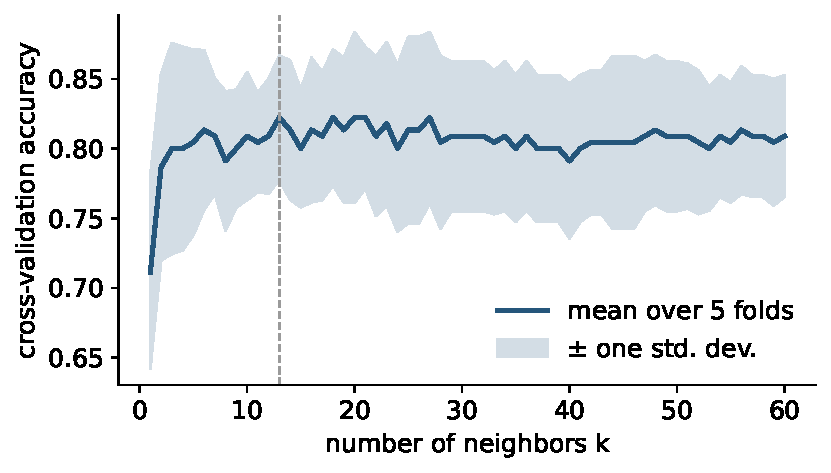
\includegraphics[width=\linewidth]{l03_gridsearch.pdf}
    \end{column}
  \end{columns}

  \note{GridSearchCV runs 5-fold cross-validation for each of the 60
    values, picks the best k, and refits it on the whole training set.
    The test accuracy of 79\% is lower than the 83\% from choosing k on the
    test set, and it is the honest number.}
\end{frame}

\begin{frame}{The full recipe}
  \vspace{0.3cm}
  \begin{enumerate}
    \item Split off a \textbf{test set}, and put it away.
    \item Choose hyperparameters with \textbf{cross-validation} on the
          training set (\texttt{GridSearchCV}).
    \item Refit the best model on the whole training set.
    \item Score it \textbf{once} on the test set, and report that number.
  \end{enumerate}

  \vfill
  \begin{takeaway}
    We use this recipe for every model in the rest of the course.
  \end{takeaway}
\end{frame}

\begin{frame}{Check your understanding}
  \begin{exercise}[three exam-style questions]
    \begin{enumerate}[itemsep=3pt,topsep=3pt]
      \item Why not choose $k$ by its accuracy on the test set?\\
            A.~it is too slow \quad
            B.~the test accuracy becomes too optimistic \quad
            C.~scikit-learn forbids it
      \item In 5-fold cross-validation, each training example is used for
            validation\\
            A.~never \quad B.~exactly once \quad C.~five times
      \item The data contain 50 schools with many students each.  The model
            must work for new schools.  Use\\
            A.~a random split \quad B.~\texttt{TimeSeriesSplit} \quad
            C.~\texttt{GroupKFold} by school
    \end{enumerate}
  \end{exercise}

  \begin{solution}
    1.~B.  2.~B.  3.~C: a school must not appear in both training and
    validation.
  \end{solution}
\end{frame}

\begin{frame}{Where this is going}
  \vspace{0.3cm}
  \begin{takeaway}
    $k$-NN predicts from similar examples.  Choose $k$ with
    cross-validation, and touch the test set only once.
  \end{takeaway}

  \vfill
  \begin{comingup}
    Lecture~4 (Tuesday, November 3): linear models for regression.
  \end{comingup}

  \vfill
  \textbf{Reading.} M\"{u}ller and Guido (2016), Chapter~2: ``Classification
  and Regression'', ``Generalization, Overfitting, and Underfitting'' and
  ``k-Nearest Neighbors''; Chapter~5: ``Cross-Validation'' and
  ``Grid Search''.
\end{frame}

\begin{frame}{References}
  \scriptsize
  \begin{itemize}
    \item M\"{u}ller, A.~C. (2017).  Applied Machine Learning, Lecture 4:
          Introduction to supervised learning (slides and notebook).
          Columbia University.
          \url{https://github.com/amueller/applied_ml_spring_2017}
    \item M\"{u}ller, A.~C. and Guido, S. (2016).  \emph{Introduction to
          Machine Learning with Python}.  O'Reilly Media.
    \item Pedregosa, F. et al. (2011).  Scikit-learn: Machine learning in
          Python.  \emph{Journal of Machine Learning Research}, 12,
          2825--2830.
    \item Rudinac, S. (2025).  Machine Learning, Lecture 3: Introduction to
          Supervised Learning.  Lecture slides, University of Amsterdam.
  \end{itemize}
\end{frame}

\end{document}
